\subsubsection*{\underline{\textsc{\Large Mummy}}}
\noindent\emph{Medium undead, lawful evil} 

Raised by dark funerary rituals and still wrapped in the shrouds of death, mummies shamble out from lost temples and tombs to slay any who disturb their rest.

\noindent\rule{0.5\textwidth}{0.5pt}

\noindent\textbf{Armor Class}: 11 (natural armor)

\noindent\textbf{Hit Points}: 58 (9d8 + 18)

\noindent\textbf{Speed}: 20 ft.

\noindent\rule{0.5\textwidth}{0.5pt}
\begin{table}[H]
	\begin{tabular}{cccccc}
		\textbf{STR} & \textbf{DEX} & \textbf{CON} & \textbf{INT} & \textbf{WIS} & \textbf{CHA} \\
		16 (+3) & 8 (-1) & 15 (+2) & 6 (-2) & 10 (+0) & 12 (+1) \\
	\end{tabular}
\end{table}
\noindent\rule{0.5\textwidth}{0.5pt}

\noindent\textbf{Saving Throws}: Wis +2

\noindent\textbf{Damage Vulnerabilities}: fire

\noindent\textbf{Damage Resistances}: bludgeoning, piercing, and slashing from non-magical attacks

\noindent\textbf{Damage Immunities}: necrotic, poison

\noindent\textbf{Condition Immunities}: charmed, exhaustion, frightened, paralyzed, poisoned

\noindent\textbf{Senses}: darkvision 60 ft., passive Perception 10

\noindent\textbf{Languages}: the languages it knew in life

\noindent\textbf{Challenge}: 3 (700 XP)

\noindent\rule{0.5\textwidth}{0.5pt}

\noindent\textbf{ACTIONS}

\noindent\textbf{Multiattack}: The mummy can use its Dreadful Glare and makes one attack with its rotting fist.

\noindent\textbf{Rotting Fist}: Melee Weapon Attack: +5 to hit, reach 5 ft., one target. Hit: 10 (2d6 + 3) bludgeoning damage plus 10 (3d6) necrotic damage. If the target is a creature, it must succeed on a DC 12 Constitution saving throw or be cursed with mummy rot. The cursed target can't regain hit points, and its hit point maximum decreases by 10 (3d6) for every 24 hours that elapse. If the curse reduces the target's hit point maximum to 0, the target dies, and its body turns to dust. The curse lasts until removed by the remove curse spell or other magic.

\noindent\textbf{Dreadful Glare}: The mummy targets one creature it can see within 60 feet of it. If the target can see the mummy, it must succeed on a DC 11 Wisdom saving throw against this magic or become frightened until the end of the mummy's next turn. If the target fails the saving throw by 5 or more, it is also paralyzed for the same duration. A target that succeeds on the saving throw is immune to the Dreadful Glare of all mummies (but not mummy lords) for the next 24 hours.

\begin{center}
	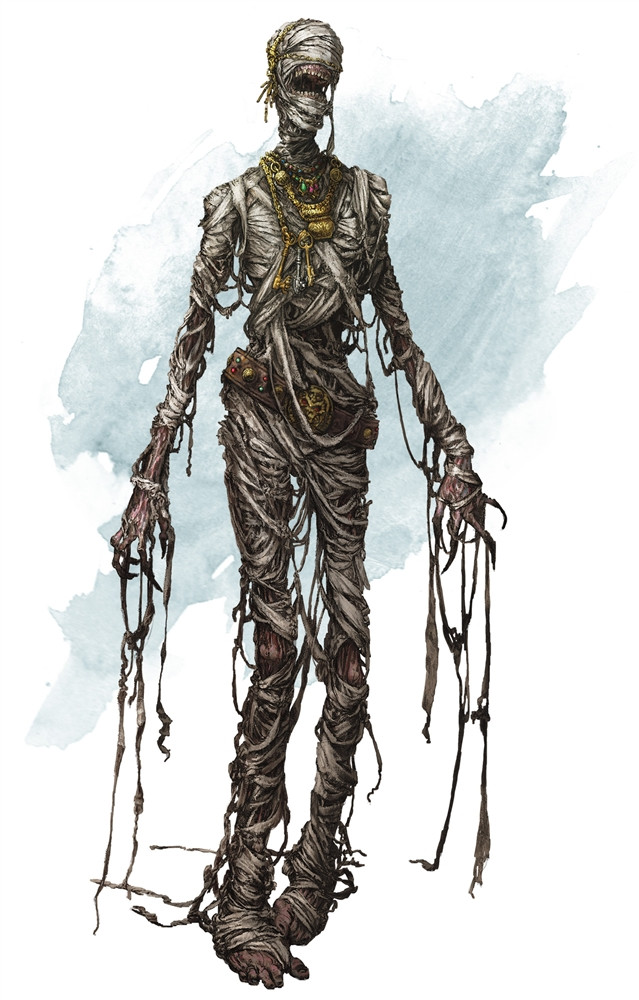
\includegraphics[width = 0.3\textwidth]{mummy}
	
	\emph{Mummy}
\end{center}